%---------------------------------------------------------------------------------
\chapter{Towards Hybrid-Duplex Multi-UAV Networks}
\label{chap:HBD_multi_UAV}
%---------------------------------------------------------------------------------
\counterwithin*{observation}{section}
\renewcommand{\theobservation}{\thesection.\arabic{observation}}

\section{Introduction}

While HBD systems have thus far been investigated to address spectrum scarcity in both manned aerial vehicle and UAV communications \cite{tan2018joint,ernest2019outage}, the analysis seen in the preceding chapters have focused on the specific case of single uplink and downlink nodes in the network. To account for any arbitrary number of uplink and downlink nodes, stochastic geometry tools need to be employed. One such stochastic geometry tool is the PPP, which is commonly used for terrestrial networks. \textcolor{black}{While PPPs have been extensively used to model the spatial locations of base stations and user equipments in cellular networks, a PPP effectively covers an infinite region \cite{chetlur2017downlink}. Furthermore, the number of nodes modeled at each instance of a PPP is not fixed. In contrast, UAV networks are more likely to be deployed over a small region with fixed numbers of deployed UAVs \cite{chetlur2017downlink,wang2018modeling}.} 

\textcolor{black}{In light of the above discussions, the BPP model is more suitable to model the spatial locations of UAVs in multi-UAV networks \cite{chetlur2017downlink,wang2018modeling}. Compared to PPPs, the BPP model allows for the area of the considered region, i.e., area of the cell, to be defined. Also, in contrast to PPPs, BPPs enable the number of deployed nodes, i.e., UAVs, at every realization to be fixed, while ensuring that the spatial locations of the nodes are uniformly distributed.} With these considerations in mind, this chapter investigates the performance of a multi-UAV network with HBD-UCS under a stochastic geometry framework.  \textcolor{black}{In particular, system models from prior chapters are extended in this chapter to incorporate the BPP model for large-scale UAV deployments}.\footnote{The work in this chapter has been published in \cite{ernest2019hybrid}.}

%%%%%%%%%%%%%%%%%%%%%%%%%%%%%%%%%%%%%%%%%%%%%%%%%%%%%%%%%%%%%%%%%%%%%%%%%%%%%%%%%%%%%%%%%%%%%%%%%%%%%%%%%%%%%%%%%%%%%%%%%%%%%%%%%%%%%%%%%
% Section 2 : System Model
\section{System Model} \label{HBD_multi_UAV_sec_sys_model}

We consider an HBD-UCS with $N_{UL}$ HD UL UAVs and one HD DL UAV communicating with a FD-GS in a suburban environment. In particular, the FD-GS receives uplink data from the $N_{UL}$ UL UAVs while simultaneously transmitting downlink data to the DL UAV. Furthermore, inter-UAV interference between the UL and DL UAVs is unavoidable due to the nature of HBD transmissions \cite{tan2018joint,ernest2019outage}. Thus, a SIC detector is considered at the DL UAV, with SI mitigation assumed at the FD-GS in this chapter. To account for the spatial deployment of UAVs, a BPP assumption is considered \cite{chetlur2017downlink, wang2018modeling}, with $D_{alt,i}^{UL}$ denoting the altitude of UL UAV-$i$ and $D_{alt,1}^{DL}$ denoting the altitude of the DL UAV. Rician fading channels are also assumed to appropriately model the propagation characteristics of the suburban environment in UAV communications \cite{matolak2017air_suburban}. Finally, the effect of Doppler shift is assumed to be compensated in this chapter \cite{tan2018joint,ernest2019outage}.

%\subsection{Distance Distribution of the UAVs}

\begin{figure} []
\centering
\vspace{-2cm}
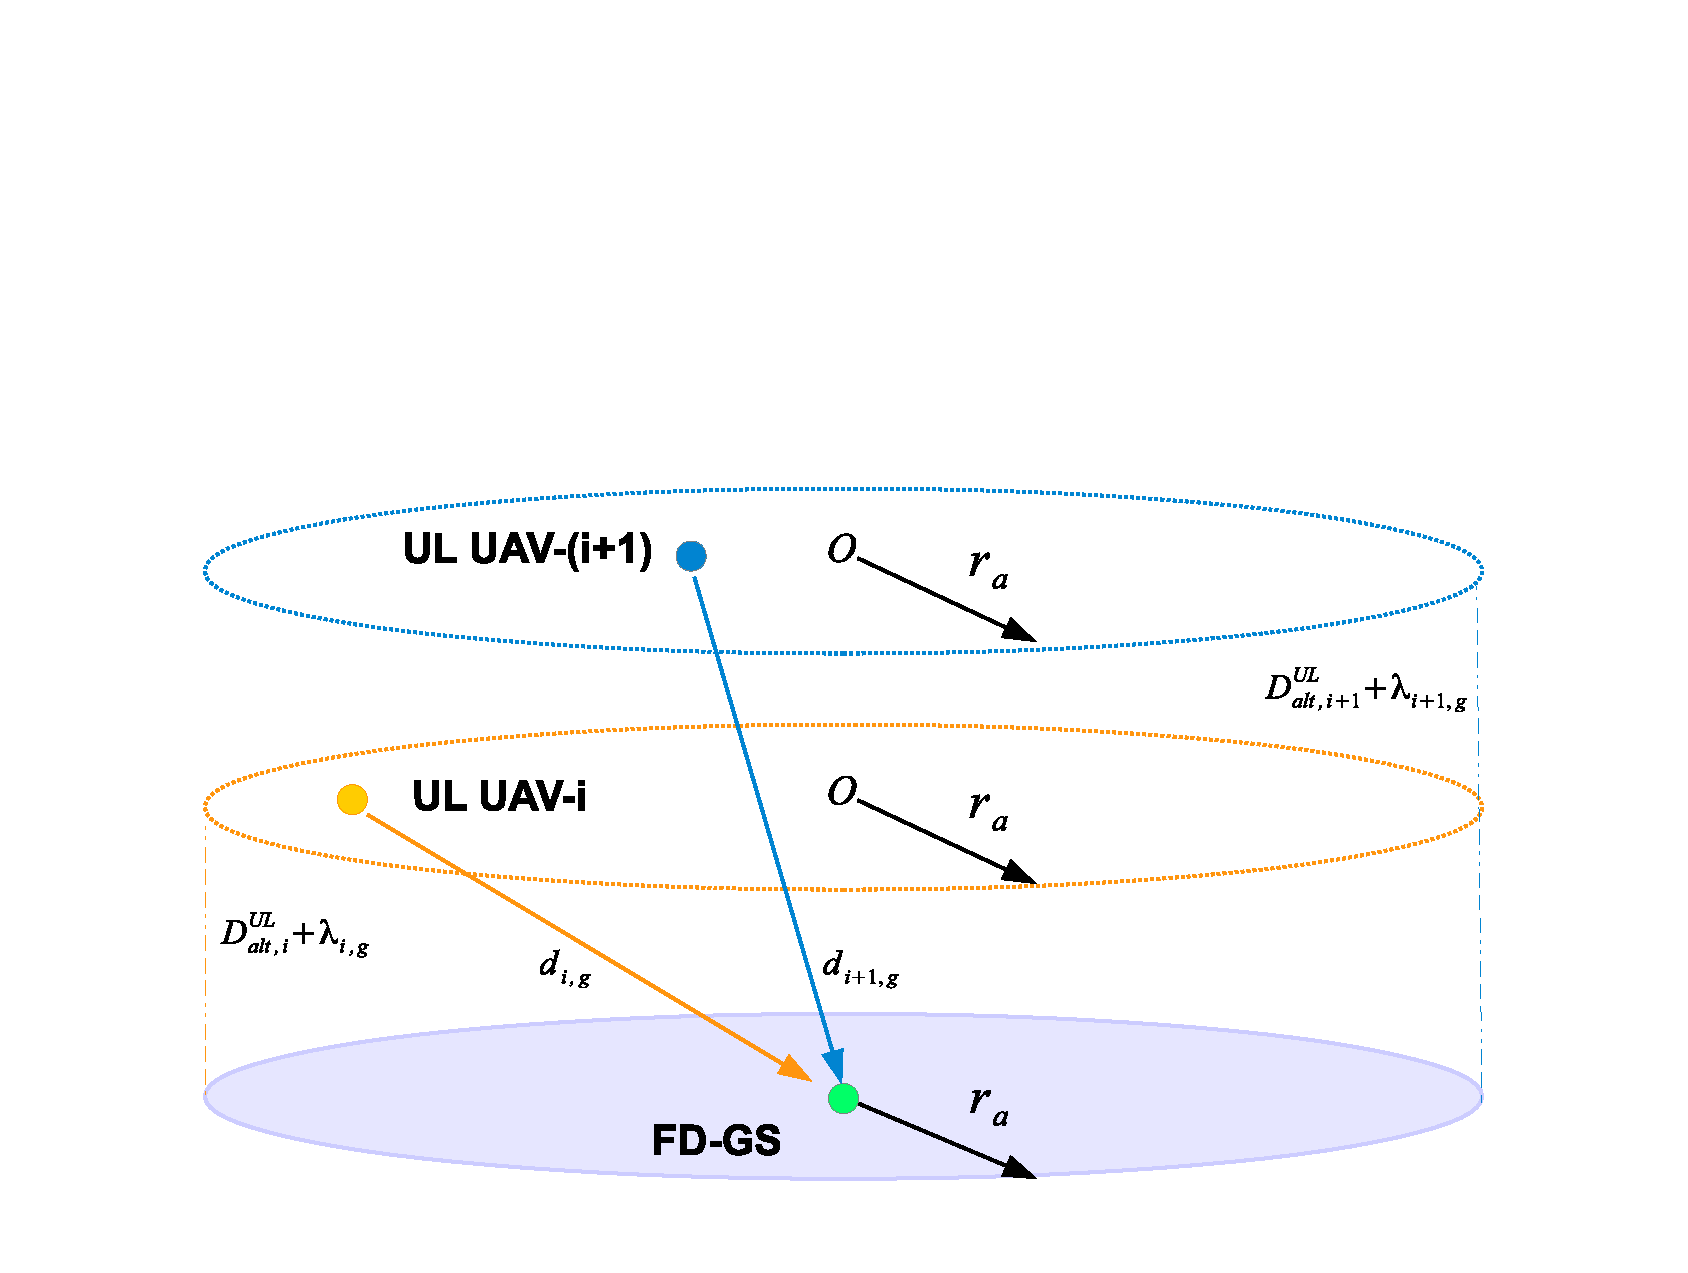
\includegraphics [width=0.6\columnwidth]{chap6_fig/UL_UAV_deployment.eps} 
%\vspace{-0.5cm}
\caption{An illustration of the UL UAV spatial locations. The spatial location of DL UAV-1 is described in the same fashion.}
\label{fig:HBD_multi_UAV_UL_UAV_deployment}
%\vspace{-0.5cm}
\end{figure}

Let the spatial location of the UAVs be uniformly distributed in a disc with radius $r_a$, angle $\left[0,2\pi\right)$, and origin $O$ above the FD-GS \cite{chetlur2017downlink}. By letting the FD-GS be located on the ground at origin $O$, we define the Euclidean distance (in km) between UL UAV-$i$ and the FD-GS as $d_{i,g}=\sqrt{D_{i,g}^2 + \big(D_{alt,i}^{UL} + \lambda_{i,g}\big)^2}$, where $D_{i,g}$ denotes the Euclidean distance between the projection of UL UAV-$i$ onto the ground plane and the FD-GS. Similarly, let the Euclidean distance between the FD-GS and DL UAV be $d_{g,1}=\sqrt{D_{g,1}^2+\big(D_{alt,1}^{DL} + \lambda_{g,1}\big)^2}$, where $D_{g,1}$ denotes the Euclidean distance between the projection of the DL UAV onto the ground plane and the FD-GS. The variable $\lambda_x$, $x \in \{(i,g),(g,1)\}$ denotes a minimum distance between the UAVs and the FD-GS such that $0 < \lambda_{x} < r_a$, $D_{alt,i}^{UL} \leq D_{alt,i+1}^{UL}$ and $\lambda_{i,g}<\lambda_{i+1,g}$, are satisfied to enable the SIC-based detection process at the FD-GS. Finally, we define the Euclidean distance between the UL and DL UAVs, i.e., inter-UAV distance, as $d_{i,1}$.

As the spatial locations of the UAVs follow a BPP, the PDF $f_{d_{x}}(w)$ of $d_{x}$ is defined as \cite[eq. (3)]{chetlur2017downlink} $f_{d_{x}}(w) =  \frac{2w}{r_a^2}$ where $x \in \{(i,g), (g,1)\}$, $D_{alt} + \lambda_{x} \leq w \leq \sqrt{ \big(D_{alt}+\lambda_{x}\big)^2+r_{a}^2}$, and $D_{alt} \in \{D_{alt,i}^{UL}, D_{alt,1}^{DL}\}$.

For the inter-UAV distance ($d_{i,1}$), the conditional PDF $f_{d_{i,1}}(w|d_{g,1})$ is given as \cite[eq. (2)]{chetlur2017downlink}:
%%%%%%%%%%%%%%%%%%%%%%%%%%%%%%%%%%%%%%%%%%%%%%%%%%%%%%%%%%%%%%%%%%%%%%%%%%%%%%%%%
\begin{eqnarray}
f_{d_{i,1}}(w|d_{g,1}) & = & \begin{cases}
		\hspace{0.25cm} \frac{2w}{r_a^2} \hspace{4.4cm}, \lambda_{i,1} \leq w \leq w_{m,1}\\
    \hspace{0.25cm} \frac{2w}{\pi r_a^2}\arccos\left( \frac{w^2 + d_{g,1}^2 - (r_a^2+\lambda_{i,1}^2)}{2d_{g,1}\sqrt{w^2 - \lambda_{i,1}^2}} \right), w_{m,1} < w \leq w_{p,1}\\ 
  \end{cases} \\\nonumber
\end{eqnarray}
%%%%%%%%%%%%%%%%%%%%%%%%%%%%%%%%%%%%%%%%%%%%%%%%%%%%%%%%%%%%%%%%%%%%%%%%%%%%%%%%%
where $w_{m,1}=\sqrt{(r_a - d_{g,1})^2 + (\lambda_{i,1})^2}$, $w_{p,1}=\sqrt{(r_a + d_{g,1})^2 + (\lambda_{i,1})^2}$, and $0 < \lambda_{i,1} <  w_{m,1}$ is the minimum distance between UL UAV-$i$ and the DL UAV. 

%Through the BPP model, a performance analysis of the HBD-UCS can be obtained with the spatial locations of the UAVs taken into consideration.

%\subsection{Received Signal at the Ground Station}

At the FD-GS, only residual SI is considered, with the SI channel modeled as a Rician fading channel to account for SI mitigation \cite{tan2018joint,ernest2019outage}. Let $x_{gs}$ and $x_i$ be the respective transmitted signals from the FD-GS and UL UAV-$i$. Then, the SOI and the SI signal at the FD-GS are $x_i$ and $x_{si}=x_{gs}$, respectively. Also, let $h_{i,g}$ denote the channel between UL UAV-$i$ and GS, and $h_{si}$ be the SI channel gain. The resultant received signal at GS can thus be written as \cite{sahai2013impact}:
%%%%%%%%%%%%%%%%%%%%%%%%%%%%%%%%%%%%%%%%%%%%%%%%%%%%%%%%%%%%%%%%%%%%%%%%%%%%%%%%%
\begin{eqnarray}
y_{gs} & = & \sum_{i=1}^{N_{UL}} \sqrt{\frac{P_i}{d_{i,g}^{n}}}h_{i,g}x_{i} + \sqrt{P_{si}} |\widetilde{h}_{si}|x_{si} + \sqrt{P_{si}}|h_{si}|\gamma_{\phi}w_{\phi} + {w_{g}}_,
\end{eqnarray} 
%%%%%%%%%%%%%%%%%%%%%%%%%%%%%%%%%%%%%%%%%%%%%%%%%%%%%%%%%%%%%%%%%%%%%%%%%%%%%%%%%
where $n$ is the pathloss exponent, $P_i$ is the transmit power of UL UAV-$i$, $P_{si}$ is the power of the SI, $\widetilde{h}_{si}$ is the error of the imperfect SI channel gain estimate, defined as $\widetilde{h}_{si}=h_{si}-\widehat{h}_{si}$, $\widehat{h}_{si}$ is the imperfect estimation of the SI channel gain, $w_{g}$ is the AWGN with zero-mean and variance $\sigma_g^2$, and $w_{\phi}$ is the Gaussian distributed phase noise with zero-mean and unit variance scaled by the strength of the phase noise $\gamma_{\phi}^2$ \cite{sahai2013impact}.\footnote{The phase noise term $\gamma_{\phi}$ reflects the jitter effect in oscillators due to hardware imperfections \cite{sahai2013impact}}

To model the worst case residual SI, the channel estimation error ($\widetilde{h}_{si}$) is modeled as a circularly symmetric zero-mean complex Gaussian random variable RV with variance $\epsilon$ \cite{tan2018joint,ernest2019outage}. Also, the total amount of SI suppression is $\frac{1}{\epsilon\sigma_g^2}$ \cite{ernest2019outage}. Finally, as $D_{alt,i}^{UL} \leq D_{alt,i+1}^{UL}$ and $\lambda_{i,g} < \lambda_{i+1,g}$, the SIC-based detection order begins from UL UAV-$i$ at the FD-GS, i.e., closest UL UAV, while treating the remaining $N_{UL}-i$ UL UAVs as interference.

%\subsection{Received Signal at the Downlink UAV}

At the DL UAV, the received signal can be written as:
%%%%%%%%%%%%%%%%%%%%%%%%%%%%%%%%%%%%%%%%%%%%%%%%%%%%%%%%%%%%%%%%%%%%%%%%%%%%%%%%%
\begin{eqnarray}
y_{DL} & = & \sqrt{\frac{P_g}{d_{g,i}^{n}}}h_{g,1}x_{gs} + \sum_{j=1}^{N_{UL}} \sqrt{\frac{P_j}{d_{j,1}^{n}}}h_{j,1}x_{j} + {w_{1}}_,
\end{eqnarray} 
%%%%%%%%%%%%%%%%%%%%%%%%%%%%%%%%%%%%%%%%%%%%%%%%%%%%%%%%%%%%%%%%%%%%%%%%%%%%%%%%%
where $P_g$ is the transmit power of the GS, $h_{g,1}$ is the channel between the FD-GS and the DL UAV, $h_{j,1}$ is the channel between UL UAV-$j$ and the DL UAV, and $w_{1}$ is the AWGN at the DL UAV with zero-mean and variance $\sigma_1^2$. As inter-UAV interference ($x_i$) is present at the DL UAV, we consider an imperfect SIC detector which removes inter-UAV interference first before detecting the SOI ($x_{gs}$). A summary of important notations is given in Table \ref{table:HBD_multi_UAV_summary_impt_notations}.

\begin{table}[]
\centering
\caption{Summary of Important Notations}
\label{table:HBD_multi_UAV_summary_impt_notations} 
\scalebox{0.8}{
\begin{tabular}{ll}
\hline
\textbf{Notations}		& \textbf{Description}																			\\  \hline \hline
$\Omega_X$						& Average received power																		\\
$\alpha_{i,j}, i\in\left\{g,1\right\}, j\in\left\{g,2\right\}, i \neq j$ & Strength of interference between $i$ and $j$				\\
$\epsilon$						& SI channel estimation error	at the FD-enabled GS					\\
$\gamma_{\phi}^2$			& Strength of phase noise at the FD- enabled GS oscillator	\\
$\sigma_g^2$					& Strength of AWGN at the FD-enabled GS											\\ 
$\sigma_2^2$					& Strength of AWGN at the UAV-2															\\ 
$r_a$ 								& Radius of the the disc 																		\\
$d_{i,1}$ 						& Euclidean distance between UL UAV-$i$ and the DL UAV 			\\
$d_{i,g}$ 						& Euclidean distance between UL UAV-$i$ and the FD-GS 			\\
$D_{alt,i}^{UL}$ 			& Altitude of UL UAV-$i$ 																		\\
$D_{alt,1}^{DL}$ 			& Altitude of the DL UAV 																		\\ 
$\lambda_x$, $x \in \{(i,g),(g,1)\}$ & Minimum distance between the UAVs and the FD-GS \\ \hline
\end{tabular}}
\end{table}
%A summary of important notations is also given in Table \ref{table:HBD_multi_UAV_summary_impt_notations}.

%%%%%%%%%%%%%%%%%%%%%%%%%%%%%%%%%%%%%%%%%%%%%%%%%%%%%%%%%%%%%%%%%%%%%%%%%%%%%%%%%%%%%%%%%%%%%%%%%%%%%%%%%%%%%%%%%%%%%%%%%%%%%%%%%%%%%%%%%
% Section 3 : Outage Probability Derivations
\section{Outage Probability} \label{HBD_multi_UAV_sec_outage}

In this section, outage probability expressions of the UL and DL UAVs are presented for the HBD-UCS. The outage probability expression for HD-UCS is also presented for benchmark comparison. Let $R^{j}_{i}$ and $R^{j}_{gs}$ for $j \in \{HBD, HD\}$ be the transmission rates of the UL UAV-$i$ and GS, respectively. For a fair comparison between the HBD-UCS and HD-UCS, we let $R_{i}^{HBD}=\frac{1}{2N_{UL}}R_{i}^{HD}$ and $R_{gs}^{HBD}=\frac{1}{2}R_{gs}^{HD}$ for uplink and downlink transmissions, respectively.

%, with sum rate defined as $R^{j}_{sum} = R^{j}_{i}+R^{j}_{gs}$

%%%%%%%%%%%%%%%%%%%%%%%%%%%%%%%%%%%%%%%%%%%%%%%%%%%%%%%%%%%%%%%%%%%%%%%%%%%%%%%%%%%%%%%%%%%%%%%%%%%%%%%%%%%%%%%%%%%%%%%%%%%%%%%%%%%%%%%%%
\subsection{Hybrid-Duplex Outage Probability}
For a SINR of $\frac{X_i d_i^{-n}}{1+\sum_{j=i+1}^{N}X_j d_j^{-n}}$ with $N$ interferers, where $X_i, 0 \leq i \leq N$ is a non-centered Chi-squared distributed random variable RV with Rician $K$ factor $K_i$, and $d_{l}^{-n}$ denotes the distance of transmitting node $l$, the outage probability is presented in the following Lemma.

\begin{lemma} \label{HBD_multi_UAV_lemma_P_out}
The outage probability $Pr\big(\mathcal{O}\big)$ for the outage event $\mathcal{O}$ at an arbitrary receiver is:
%%%%%%%%%%%%%%%%%%%%%%%%%%%%%%%%%%%%%%%%%%%%%%%%%%%%%%%%%%%%%%%%%%%%%%%%%%%%%%%%%
\begin{eqnarray} 
Pr\big(\mathcal{O}\big) & \approx & \sum_{q=0}^{K_{tr}} \sum_{l_1+\ldots+l_{N-q+1}=q+1} \alpha\big(q,\overline{P}_i,K_{i},\gamma\big) \binom{l_1 + \ldots + l_{N-q+1}}{l_1,\ldots, l_{N-q+1}} \nonumber \\
 & & \times \int_{-\infty}^{\infty} w_i^{n(q+1)}f_{d_i}(w_i) \Bigg( \prod_{j=1}^{N-i} E\Big\{X_{j}^{l_j}\Big\} \int_{-\infty}^{\infty} w_j^{-nl_j}f_{d_j}(w_j) dw_j \Bigg)  {dw_i}_,
\end{eqnarray}
%%%%%%%%%%%%%%%%%%%%%%%%%%%%%%%%%%%%%%%%%%%%%%%%%%%%%%%%%%%%%%%%%%%%%%%%%%%%%%%%%
\end{lemma}
where $\mathcal{O}=\Big\{ X_{i}, X_{j} : R \geq \log_{2}\Big(1 + \frac{X_i d_i^{-n}}{1+\sum_{j=i+1}^{N}X_j d_j^{-n}}\Big)\Big\}$, $R$ is the transmission rate, $K_{tr}$ is the truncation order, $\alpha\big(q,\overline{P}_i,K_i,\gamma\big) = (-1)^q \exp(-K_i) \frac{{L_q}^{(i)}(K_i)}{(1+q)!} \Big(\frac{(1+K_i)}{\overline{P}_i}\gamma\Big)^{q+1}$ is the CDF expansion of the RV $X_i$, $\overline{P}_i$ is the variance of $X_i$, $\gamma$ is the threshold, ${L_q}^{(0)}(\bullet)$ is the $q$-th degree, zero-order Laguerre polynomials \cite{tan2018joint, ernest2019outage}, and $E\{\bullet\}$ is the statistical expectation. Also, $E\Big\{X_{j}^{l_j}\Big\}=\Gamma(1+l_j) \left[\frac{\overline{P}_j}{1+K_{j}}\right]^{l_j} {}_1{F_1}(-l_j,1;-K_{j})$ is the $l_j^{th}$ moment of $X_j$ \cite[eq. (7)]{ernest2019outage} with ${}_1{F_1}(\bullet)$ representing the confluent Hypergeometric function \cite{ernest2019outage}.

\begin{proof}
The proof is provided in Appendix \ref{HBD_multi_UAV_lemma_P_out_proof}.
\end{proof} 

From Lemma \ref{HBD_multi_UAV_lemma_P_out}, the outage probability expressions of the UL and DL UAVs can be obtained.

\subsubsection{Uplink UAV-$i$}
Let $X_{i,g}=P_{i,g}|h_{i,g}|^2$ be the instantaneous received power of the SOI from UL UAV-$i$ at the FD-GS, where $P_{i,g}=\frac{P_i}{\sigma_g^2}$. Also, let $Y_{si,1}=P_{si}\gamma_{\phi}^2|h_{si}|^2$ and $Y_{si,2}=P_{si}\epsilon|\widetilde{h}_{si}|^2$ be the instantaneous received power of the residual SI components, where $P_{si}=P_{i,g}$. The symbols $X_{i,g}$ and $Y_{si,1}$ are non-centered Chi-squared distributed RVs with respective Rician $K$ factors $K_{i,g}$ and $K_{si,1}$ while $Y_{si,2}$ is an exponentially distributed RV. Defining the outage event of UL UAV-$i$ as $\mathcal{O}_{UL,i}^{HBD} = \Big\{ h_{i,g}, h_{si} : R_{i}^{HBD} \geq \log_{2}\Big(1 + \frac{X_{i,g}d_{i,g}^{-n}}{\sum_{j=i+1}^{N_{UL}} X_{j,g}d_{j,g}^{-n} + Y_{si,1} + Y_{si,2} + 1}\Big)\Big\}$, with threshold $\gamma_{gs}^{HBD} = 2^{R_{i}^{HBD}}-1$, the outage probability $Pr\big(\mathcal{O}_{UL,i}^{HBD}\big)$ of UL UAV-$i$ is presented in the following theorem:

\begin{theorem} \label{HBD_multi_UAV_theorem_P_out_UL_uav_i}
%%%%%%%%%%%%%%%%%%%%%%%%%%%%%%%%%%%%%%%%%%%%%%%%%%%%%%%%%%%%%%%%%%%%%%%%%%%%%%%%%
The outage probability at UL UAV-$i$ is
\begin{eqnarray} \label{HBD_multi_UAV_P_out_UL_uav_i}
Pr\big(\mathcal{O}_{UL,i}^{HBD}\big) & \approx & \sum_{q=0}^{K_{tr}} \sum_{l_1+\ldots+l_{N_{UL}-i+3}=q+1} \alpha\big(q,P_{i,g},K_{i,g},\gamma_{gs}^{HBD}\big) \Delta\big(D_{alt,i}^{UL},\lambda_{i,g},q\big) \nonumber\\ 
& & \hspace{-1cm} \times \binom{l_1 + \ldots + l_{N_{UL}-i+3}}{l_1,\ldots, l_{N_{UL}-i+3}} E\Big\{Y_{si,1}^{l_1}\Big\} E\Big\{Y_{si,2}^{l_2}\Big\} \prod_{j=1}^{N_{UL}-i} E\Big\{X_{j,g}^{l_j}\Big\} \overline{\Delta}\big(D_{alt,j}^{UL},\lambda_{j,g},l_j\big)_,
\end{eqnarray}
%%%%%%%%%%%%%%%%%%%%%%%%%%%%%%%%%%%%%%%%%%%%%%%%%%%%%%%%%%%%%%%%%%%%%%%%%%%%%%%%%
where $n \neq 2$, $\Delta\big(D_{alt,i}^{UL},\lambda_{i,g},q\big) = \frac{2}{[n(q+1)+2]r_a^2} \Big( \big[\big(D_{alt,i}^{UL} + \lambda_{i,g}\big)^2 + r_a^2 \big]^{\frac{n(q+1)+2}{2}} - \big[\big(D_{alt,i}^{UL} + \lambda_{i,g}\big)^2 \big]^{\frac{n(q+1)+2}{2}} \Big)$, and $\overline{\Delta}\big(D_{alt,j}^{UL},\lambda_{j,g},l_j\big) = \frac{2}{[2-nl_j]r_a^2} \Big( \big[\big(D_{alt,j}^{UL} + \lambda_{j,g}\big)^2 + r_a^2 \big]^{\frac{2-nl_j}{2}} - \big[\big(D_{alt,j}^{UL} + \lambda_{j,g}\big)^2  \big]^{\frac{2-nl_j}{2}} \Big)$.
\end{theorem}
\begin{proof}
Applying Lemma \ref{HBD_multi_UAV_lemma_P_out} and integrating the resulting expression over the PDFs $f_{d_{i,g}}(w_i)$ and $f_{d_{j,g}}(w_j)$ yields Theorem \ref{HBD_multi_UAV_theorem_P_out_UL_uav_i}.
\end{proof}

As $2-nl_j$ is present in the denominator of $\overline{\Delta}\big(D_{alt,j}^{UL},\lambda_{j,g},l_j\big)$, Theorem \ref{HBD_multi_UAV_theorem_P_out_UL_uav_i} is valid only when $n \neq 2$. However, it must be noted that selecting $n \approx 2$, e.g., $n = 2 + 10^{-6}$, enables Theorem \ref{HBD_multi_UAV_theorem_P_out_UL_uav_i} to be applied for outage probability analysis involving free space path loss scenarios.\footnote{Selecting $n \approx 2$, e.g., $n = 2 + 10^{-6}$, allows $\overline{\Delta}\big(D_{alt,j}^{UL},\lambda_{j,g},l_j\big)$ to be evaluated for free space path loss scenarios while avoiding a zero in the denominator.} \textcolor{black}{\footnote{\textcolor{black}{To analytically ascertain the accuracy of the new power series expressions in this chapter, one will need to conduct a truncation analysis. Work in this direction is left as an open research challenge which can be addressed in future studies.}}}

\subsubsection{Downlink UAV}

At the DL UAV, let $X_{g,1}=P_{g,1}|h_{g,1}|^2$ be the instantaneous received power of the SOI from the GS at the DL UAV, where $P_{g,1}=\frac{P_g}{\sigma_1^2}$. Also, let $X_{j,1}=P_{j,1}\beta_{j,1}|h_{j,1}|^2$ be the instantaneous received powers of the inter-UAV interference from UL UAV-$j$ due to HBD transmissions, where $P_{j,1}=\frac{P_j}{\sigma_1^2}$, and $0 \leq \beta_{j,1} \leq 1$ denotes the strength of the residual interference due to imperfect SIC. The symbols $X_{g,1}$ and $X_{j,1}$ are non-centered Chi-squared distributed RVs with respective Rician $K$ factors $K_{g,1}$ and $K_{j,1}$. Defining the outage event at the DL UAV as $\mathcal{O}_{DL}^{HBD} = \Big\{ h_{g,1}, h_{j,1} : R_{gs}^{HBD} \geq \log_{2}\Big(1 + \frac{X_{g,1}d_{g,1}^{-n}}{\sum_{j=1}^{N_{UL}}X_{j,1}d_{j,1}^{-n} + 1}\Big)\Big\}$, the outage probability expression for the DL UAV is presented in the following theorem.

\begin{theorem} \label{HBD_multi_UAV_theorem_P_out_DL_uav}
%%%%%%%%%%%%%%%%%%%%%%%%%%%%%%%%%%%%%%%%%%%%%%%%%%%%%%%%%%%%%%%%%%%%%%%%%%%%%%%%%
The HBD outage probability at the DL UAV is
\begin{eqnarray} \label{HBD_multi_UAV_P_out_DL_uav}
Pr\big(\mathcal{O}_{DL}^{HBD}\big) & \approx & \sum_{q=0}^{K_{tr}} \sum_{l_1+\ldots+l_{N_{UL}+1}=q+1} \alpha\big(q,P_{g,1},K_{g,1},\gamma_{DL}^{HBD}\big) \binom{l_1 + \ldots + l_{N_{UL}-i+3}}{l_1,\ldots, l_{N_{UL}-i+3}} \nonumber\\ 
 & & \hspace{0.5cm} \times \int_{L_1}^{L_2} \frac{2w_{g,1}^{n(q+1)+1}}{r_a^2} \Bigg( \prod_{j=1}^{N_{UL}} E\Big\{X_{j,1}^{l_j}\Big\} \Xi_{j,1}(w_{g,1},l_j) \Bigg){dw_{g,1}}_,
\end{eqnarray}
%%%%%%%%%%%%%%%%%%%%%%%%%%%%%%%%%%%%%%%%%%%%%%%%%%%%%%%%%%%%%%%%%%%%%%%%%%%%%%%%%
where $L_1 = D_{alt,1}^{DL} + \lambda_{g,1}$, $L_2 = \sqrt{\big(D_{alt,1}^{DL} + \lambda_{g,1}\big)^2 + r_{a}^2}$, $\gamma_{DL}^{HBD} = 2^{R_{gs}^{HBD}}-1$, and $\Xi_{j,1}(w_{g,1},l_j) = \frac{2\big[(w_{m,1})^{2-nl_j} - \lambda_{j,1}^{2-nl_j}\big]}{r_a^2[2-nl_j]} + \int_{w_{m,1}}^{w_{p,1}} \frac{2w_{j,1}}{\pi r_a^2}\arccos\Bigg( \frac{w_{j,1}^2 + w_{g,1}^2 - (r_a^2+\lambda_{j,1}^2)}{2w_{g,1}\sqrt{w_{j,1}^2 - \lambda_{j,1}^2}} \Bigg) {dw_{j,1}}$.
%%%%%%%%%%%%%%%%%%%%%%%%%%%%%%%%%%%%%%%%%%%%%%%%%%%%%%%%%%%%%%%%%%%%%%%%%%%%%%%%%%
%\begin{eqnarray}
%\Xi_{j,1}(w_{g,1},l_j) & = & \frac{2\big[(w_{m,1})^{2-nl_j} - \lambda_{j,1}^{2-nl_j}\big]}{r_a^2[2-nl_j]} \nonumber \\
 %& & \hspace{-2.7cm} + \int_{w_{m,1}}^{w_{p,1}} \frac{2w_{j,1}}{\pi r_a^2}\arccos\Bigg( \frac{w_{j,1}^2 + w_{g,1}^2 - (r_a^2+\lambda_{j,1}^2)}{2w_{g,1}\sqrt{w_{j,1}^2 - \lambda_{j,1}^2}} \Bigg) {dw_{j,1}}_.
%\end{eqnarray}
%%%%%%%%%%%%%%%%%%%%%%%%%%%%%%%%%%%%%%%%%%%%%%%%%%%%%%%%%%%%%%%%%%%%%%%%%%%%%%%%%%
\end{theorem}
\begin{proof}
Theorem \ref{HBD_multi_UAV_theorem_P_out_DL_uav} is proven using the same approach in Theorem \ref{HBD_multi_UAV_theorem_P_out_UL_uav_i}.
\end{proof}

%With (\ref{P_out_UL_uav_i}) and (\ref{P_out_DL_uav}), a stochastic geometry-based outage probability analysis of the HBD-UCS over Rician fading UAV channels is now possible. 

%%%%%%%%%%%%%%%%%%%%%%%%%%%%%%%%%%%%%%%%%%%%%%%%%%%%%%%%%%%%%%%%%%%%%%%%%%%%%%%%%%%%%%%%%%%%%%%%%%%%%%%%%%%%%%%%%%%%%%%%%%%%%%%%%%%%%%%%%
\subsection{Half-Duplex Outage Probability}
We compare the HBD-UCS with HD-UCS as a benchmark scheme. For the HD-UCS, an outage is declared for UL UAV-$i$ when $R_{i}^{HD} \geq \log_{2}\big(1 + X_{i,g}d_{i,g}^{-n}\big)$. Similarly, an outage is declared for the DL UAV when $R_{gs}^{HD} \geq \log_{2}\big(1 + X_{g,1}d_{g,1}^{-n}\big)$. Thus, the HD-UCS outage events for UL UAV-$i$ and the DL UAV are defined as $\mathcal{O}_{UL,i}^{HD} = \big\{ h_{i,g} : R_{i}^{HD} \geq \log_{2}\big(1 + X_{i,g}d_{i,g}^{-n}\big)\big\}$ and $\mathcal{O}_{DL}^{HD} = \Big\{ h_{g,1} : R_{gs}^{HD} \geq \log_{2}\Big(1 + X_{g,1}d_{g,1}^{-n}\Big)\Big\}$, respectively. Following the same approach presented in Appendix \ref{HBD_multi_UAV_lemma_P_out_proof}, the HD-UCS outage probability expressions for UL UAV-$i$ and the DL UAV are:
%%%%%%%%%%%%%%%%%%%%%%%%%%%%%%%%%%%%%%%%%%%%%%%%%%%%%%%%%%%%%%%%%%%%%%%%%%%%%%%%%%
\begin{eqnarray}
 Pr\big(\mathcal{O}_{UL,i}^{HD}) & \hspace{-0.1cm} \approx & \hspace{-0.1cm} \sum_{q=0}^{K_{tr}} \alpha\big(q,P_{i,g},K_{i,g},\gamma_{gs}^{HD}\big) \Delta\big(D_{alt,i}^{UL},\lambda_{i,g},q\big)_, \\
 Pr\big(\mathcal{O}_{DL}^{HD}) & \hspace{-0.1cm} \approx & \hspace{-0.1cm} \sum_{q=0}^{K_{tr}} \alpha\big(q,P_{g,1},K_{g,1},\gamma_{DL}^{HD}\big) \Delta\big(D_{alt,1}^{DL},\lambda_{g,1},q\big)_,
\end{eqnarray}
%%%%%%%%%%%%%%%%%%%%%%%%%%%%%%%%%%%%%%%%%%%%%%%%%%%%%%%%%%%%%%%%%%%%%%%%%%%%%%%%%%
where $\gamma_{gs}^{HD} = 2^{R_{1}^{HD}}-1$ and $\gamma_{DL}^{HD} = 2^{R_{gs}^{HD}}-1$.

%%%%%%%%%%%%%%%%%%%%%%%%%%%%%%%%%%%%%%%%%%%%%%%%%%%%%%%%%%%%%%%%%%%%%%%%%%%%%%%%%%%%%%%%%%%%%%%%%%%%%%%%%%%%%%%%%%%%%%%%%%%%%%%%%%%%%%%%%
% Section 4: Numerical Results
\section{Numerical Results} \label{HBD_multi_UAV_sec_num_res}

The outage probability of the HBD-UCS is analyzed in this section for Rician $K$ factors of 10 dB \cite[Table V]{matolak2017air_suburban}, $0\text{ dB} \leq P_t \leq 30\text{ dB}$, $P_{i,g} = P_{g,1} = P_{j,1} = P_t$, $\sigma_g^2 = \sigma_{1}^2 = -131\text{dBm}$ \cite{itu2011m2233}, $R_{x}^{HD} =  0.1 \text{b/s/Hz}, i \in \{i,gs\}$, $\gamma_{\phi}^2 = -140\text{dBm}$, $\epsilon=0.01$ \cite{ernest2019outage}, $r_a=4$ km, $n \approx 2$ \cite[Table III]{matolak2017air_suburban}, $N_{UL}=3$, $\lambda_{1,g} =1.3$, $\lambda_{2,g} =1.4$, $\lambda_{3,g} =1.5$, $\beta_{j,1}=0.5^2$, and Monte Carlo simulations using $10^{5}$ samples.

\begin{figure*}[h]
\centering
%\vspace{-0.5cm}
\subfloat[Uplink outage probability.]{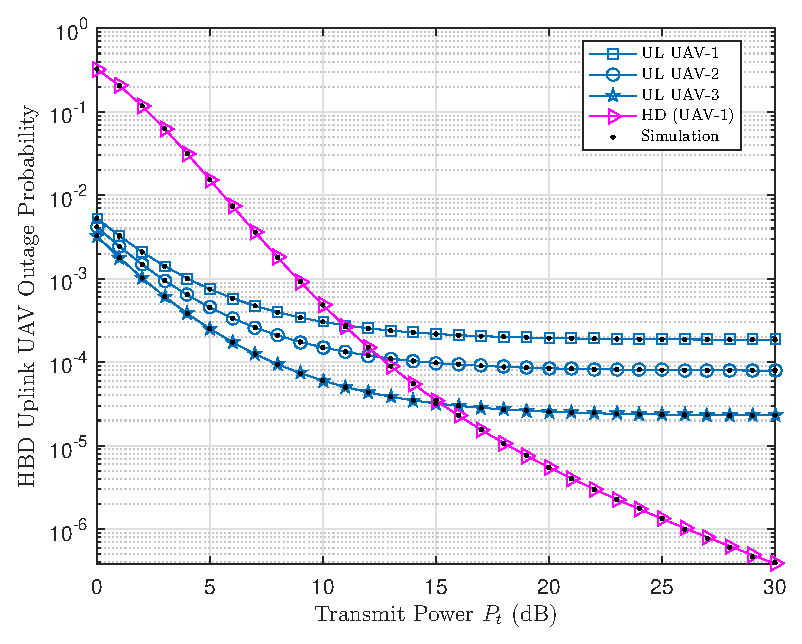
\includegraphics [width=0.45\columnwidth]{chap6_fig/hbd_UL_outage.eps}
\label{fig:HBD_multi_UAV_pout_UL}}
\hfil
\subfloat[Downlink outage probability for $\lambda_{1,1} = 1.4$, $\lambda_{2,1} = 1.3$, and $\lambda_{3,1} = 1.2$.]{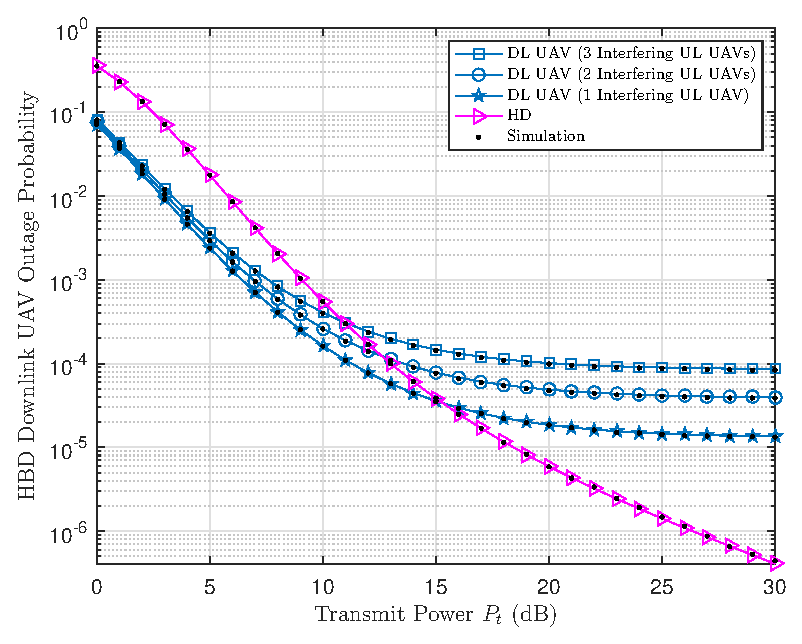
\includegraphics [width=0.45\columnwidth]{chap6_fig/hbd_DL_outage.eps}
\label{fig:HBD_multi_UAV_pout_DL}}
\hfil
\subfloat[Impact of SI cancellation and phase noise on uplink outage probability.]{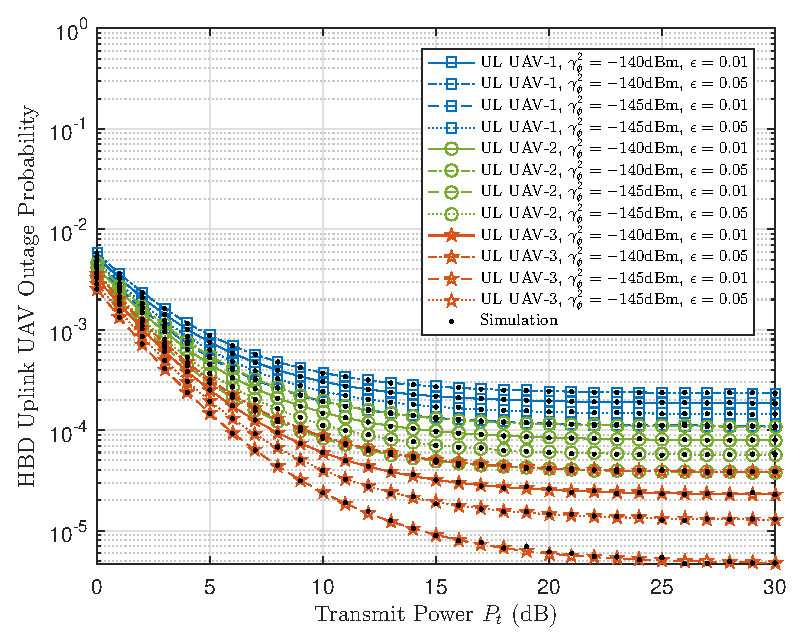
\includegraphics [width=0.45\columnwidth]{chap6_fig/hbd_UL_outage_SI_cancellation.eps}
\label{fig:HBD_multi_UAV_pout_SI_cancellation}}
\caption{Outage probability of the HBD-UCS.}
\label{fig:HBD_multi_UAV_pout}
%\vspace{-0.51cm}
\end{figure*}

%%%%%%%%%%%%%%%%%%%%%%%%%%%%%%%%%%%%%%%%%%%%%%%%%%%%%%%%%%%%%%%%%%%%%%%%%%%%%%%%%%
% At low $P_t$ regimes, the HBD-UCS outperforms the HD-UCS in terms of uplink and downlink outage probability. 
% Additionally, for uplink transmissions, recall that the FD-GS detects UL UAV-$i$ by treating the remaining $N_{UL}-i$ UL UAVs as interference. As such, UL UAV-1 is seen to exhibit higher outage probability then UL UAV-2 and UAV-3, with similar observations also noted for the subsequent UL UAVs.
% It is also seen that, depending on the number of interfering UL UAVs, the HBD-UCS can also attain lower downlink outage probability than the HD-UCS at moderate $P_t$ regimes, e.g., $N_{UL}\in \{2,3\}$.
% At high $P_t$ regimes, the HD-UCS attains lower outage probability than the HBD-UCS for both uplink and downlink outage probability. 
% For uplink transmissions, error floors are observed since the detection process at the FD-GS becomes interference-limited due to interference from the remaining $N_{UL}-i$ UL UAVs. Similarly, for downlink transmissions, error floors are observed due to the downlink UAV becoming interference-limited as a result of residual SIC interference. 
% Thus, it is shown that the HBD-UCS is well suited for multi-UAV networks since UAV communications operate at low $P_t$ regimes. \footnote{It is worth noting that UAVs largely operate at low $P_t$ regimes due to SWAP restrictions. For instance, $29\text{dBm} \leq P_t \leq 40\text{dBm}$ was noted in \cite{ITU2011}, while in \cite{zeng2018cellularconnecteduav}, cellular-to-UAV links were evaluated for $P_t = 20\text{dBm}$. The values found in \cite{ITU2011,zeng2018cellularconnecteduav} translates into $-10 \text{dB} \leq P_t \leq 10 \text{dB}$.}
%%%%%%%%%%%%%%%%%%%%%%%%%%%%%%%%%%%%%%%%%%%%%%%%%%%%%%%%%%%%%%%%%%%%%%%%%%%%%%%%%%

\begin{observation}
\emph{\emph{With effective SI mitigation, the HBD-UCS achieves lower outage probability at low $P_t$ regimes than the HD-UCS and is able to fulfill $PER$ requirements for CNPC links in LTE networks.}}
\end{observation}

The outage probability of the HBD-UCS is compared against the HD-UCS for both UL and DL transmissions in Fig. \ref{fig:HBD_multi_UAV_pout}. At low $P_t$ regimes, the HBD-UCS outperforms the HD-UCS in terms of UL and DL outage probability. In particular, the HBD-UCS is able to fulfill $PER$ requirements for UAV control links over Long Term Evolution (LTE) networks, i.e., $PER<10^{-3}$ \cite{tr362017}.\footnote{Outage probability can be used to represent $PER$ if the transmitted signals span over one fading block \cite{ernest2019outage}.} Additionally, for UL transmissions, recall that the FD-GS detects UL UAV-$i$ by treating the remaining $N_{UL}-i$ UL UAVs as interference. As such, UL UAV-1 is seen to exhibit higher outage probability than UL UAV-2 and UAV-3, with similar observations also noted for the subsequent UL UAVs. It is also seen that, depending on the number of interfering UL UAVs, the DL UAV can also attain lower DL outage probability than the HD-UCS at moderate $P_t$ regimes, e.g., $N_{UL}\in \{2,3\}$. 

At high $P_t$ regimes, the HD-UCS attains lower outage probability than the HBD-UCS for both UL and DL outage probability. For UL transmissions, error floors are observed since the detection process at the FD-GS becomes interference-limited due to interference from the remaining $N_{UL}-i$ UL UAVs. Similarly, for DL transmissions, error floors are observed due to the DL UAV becoming interference-limited as a result of residual SIC interference.  Thus, it is shown that the HBD-UCS is well suited for multi-UAV networks since UAV communications operate at low $P_t$ regimes.\footnote{It is worth noting that UAVs largely operate at low $P_t$ regimes due to size, weight, and power restrictions. For instance, $29\text{dBm} \leq P_t \leq 40\text{dBm}$ was noted in \cite{itu2011m2233}, while in \cite{zeng2018cellularconnecteduav}, cellular-to-UAV links were evaluated for $P_t = 20\text{dBm}$. The values found in \cite{itu2011m2233,zeng2018cellularconnecteduav} translates into $-10 \text{dB} \leq P_t \leq 10 \text{dB}$.}\footnote{Outage probability can be further reduced when the transmit power and trajectory of the UAVs are optimized iteratively. For transmit power optimization, one should consider the spatial location of the UAVs and the trajectory. For trajectory optimization, both the spiral and oval trajectory processes should be considered to maintain a uniform distribution under the BPP model \cite{enayati2019moving}.} The impact of SI cancellation and phase noise on uplink outage probability is seen in Fig. \ref{fig:HBD_multi_UAV_pout_SI_cancellation}. It is observed that an increase in either $\gamma_{\phi}^2$ or $\epsilon$ causes the outage probability of the UL UAVs to increase. Furthermore, an increasing $\gamma_{\phi}^2$ causes higher outage probability than an increasing $\epsilon$ due to higher residual SI at the FD-GS. Thus, the reliability of UL UAV transmissions in an HBD-UCS hinges on having effective SI mitigation architectures with low phase noise FD transceivers at the GS. 

\begin{figure}[]
\centering
\subfloat[Uplink outage probability.]{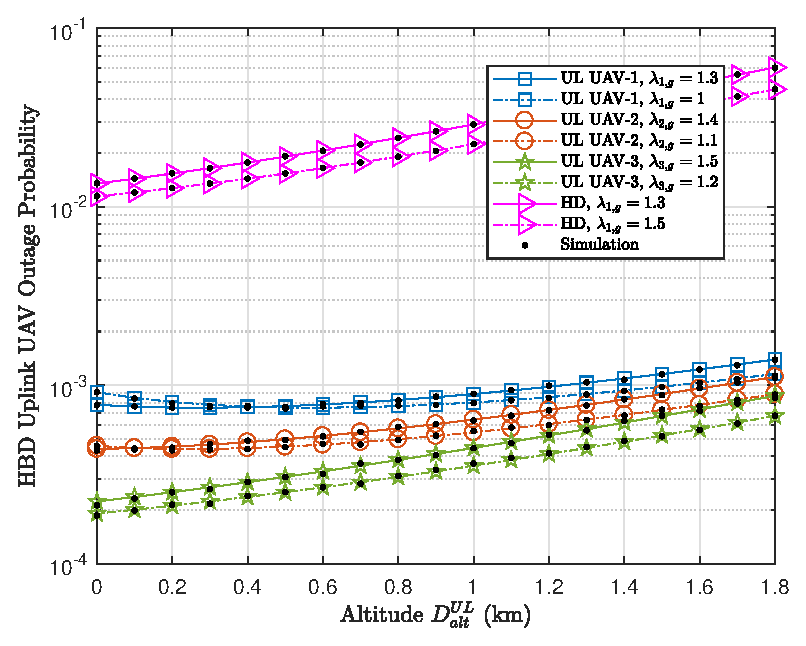
\includegraphics [width=0.45\columnwidth]{chap6_fig/hbd_UL_outage_height.eps}
\label{fig:HBD_multi_UAV_hbd_UL_outage_height}} 
\hfil
\subfloat[Downlink outage probability.]{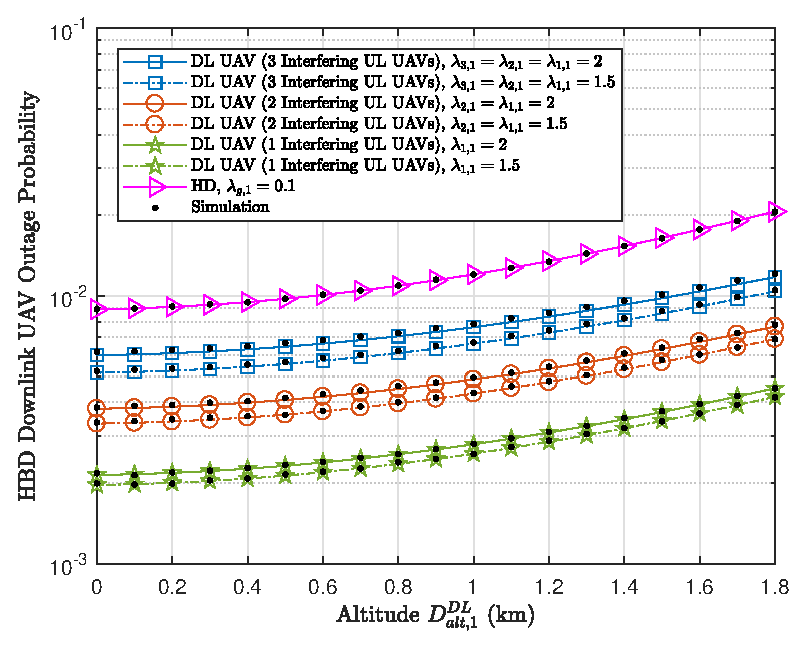
\includegraphics [width=0.45\columnwidth]{chap6_fig/hbd_DL_outage_height.eps}
\label{fig:HBD_multi_UAV_hbd_DL_outage_height}}
\caption{Impact of height and minimum distance on the outage probability of the HBD-UCS at $P_t = 5$ dB, $\beta = 1$, $\lambda_{g,1} = 0.1$, and $D_{alt}^{UL}=D_{alt,i}^{UL}$.}
\label{fig:HBD_multi_UAV_pout_height}
%\vspace{-0.6cm}
\end{figure}

%%%%%%%%%%%%%%%%%%%%%%%%%%%%%%%%%%%%%%%%%%%%%%%%%%%%%%%%%%%%%%%%%%%%%%%%%%%%%%%%%%
% In Fig. \ref{fig:pout_height}, the impact of height and minimum distance on the outage probability of the HBD-UCS is analyzed.
% For UL transmissions, a lower outage probability is attained when $ 0 \leq D_{alt}^{UL} \leq 1$ and $\lambda_{i,g}$ is reduced, since weaker UL interference is experienced. However, when $D_{alt}^{UL} > 1$, outage probability increases due to a weaker SOI. Similarly, increasing $\lambda_{i,g}$ leads to higher outage probability as the SOI is further weakened. 
% For DL transmissions, increasing $D_{alt,1}^{DL}$ leads to higher outage probability for the HBD-UCS and HD-UCS due to a weaker SOI. It is also observed that increasing $\lambda_{i,1}$ reduces outage probability since inter-UAV interference is weakened. 
% Therefore, as seen in Fig. \ref{fig:pout_height}, one may have to consider other approaches if support for UAVs deployed at high altitudes is required. Nonetheless, Fig. \ref{fig:pout} and Fig. \ref{fig:pout_height} have demonstrated that the multi-UAV network with HBD-UCS is able to support more UAVs concurrently on the same spectrum while attaining a lower outage probability than the HD-UCS.
%%%%%%%%%%%%%%%%%%%%%%%%%%%%%%%%%%%%%%%%%%%%%%%%%%%%%%%%%%%%%%%%%%%%%%%%%%%%%%%%%%

\begin{observation}
\emph{\emph{Increasing the altitude of the UAVs leads to higher outage probability for the HBD-UCS.}}
\end{observation}

In Fig. \ref{fig:HBD_multi_UAV_pout_height}, the impact of height and minimum distance on the outage probability of the HBD-UCS is analyzed. For UL transmissions, a lower outage probability is attained when $ 0 \leq D_{alt}^{UL} \leq 1$ and \textcolor{black}{when} $\lambda_{i,g}$ is reduced, since weaker UL interference is experienced. However, when $D_{alt}^{UL} > 1$, outage probability increases due to a weaker SOI. Similarly, increasing $\lambda_{i,g}$ leads to higher outage probability as the SOI is further weakened. For DL transmissions, increasing $D_{alt,1}^{DL}$ leads to higher outage probability for the HBD-UCS and HD-UCS due to a weaker SOI. It is also observed that increasing $\lambda_{i,1}$ reduces outage probability since inter-UAV interference is weakened. Therefore, as seen in Fig. \ref{fig:HBD_multi_UAV_pout_height}, one may have to consider other approaches if support for UAVs deployed at high altitudes is required. Nonetheless, Fig. \ref{fig:HBD_multi_UAV_pout} and Fig. \ref{fig:HBD_multi_UAV_pout_height} have demonstrated that the multi-UAV network with HBD-UCS is able to support more UAVs concurrently on the same spectrum while attaining a lower outage probability than the HD-UCS.

%%%%%%%%%%%%%%%%%%%%%%%%%%%%%%%%%%%%%%%%%%%%%%%%%%%%%%%%%%%%%%%%%%%%%%%%%%%%%%%%%%%%%%%%%%%%%%%%%%%%%%%%%%%%%%%%%%%%%%%%%%%%%%%%%%%%%%%%%
% Section 5: Conclusion
\section{Chapter Summary} \label{HBD_multi_UAV_sec_conclusion}

In this chapter, the outage probability analysis of a multi-UAV network with HBD-UCS is investigated within a stochastic geometry framework. It is demonstrated that at low transmit power regimes, the HBD-UCS achieves lower outage probability than the HD-UCS for both uplink and downlink transmissions. It is also shown that the HBD-UCS can support uplink and downlink transmissions that are more reliable than the HD-UCS, when the UAV operating altitude is increased. Thus, we demonstrate that the HBD-UCS is able to concurrently support more UAVs while achieving a higher reliability than the HD-UCS.

To enable a greater number of deployed UAVs in multi-UAV networks with ease of deployment, one can consider tapping on existing cellular infrastructure to support multi-UAV communications. In this spirit, NOMA-aided multi-UAV communications is examined in the next chapter for FD heterogeneous networks. 




\counterwithin*{observation}{subsection}
\renewcommand{\theobservation}{\thesubsection.\arabic{observation}}


